\documentclass[red, hyperref={pdfpagelabels=false}]{beamer}
%\hypersetup{pdfpagemode=FullScreen}

\mode<presentation>
\usepackage{beamerthemesplit}
\usepackage[T1]{fontenc}
\usepackage{textcomp}
\usepackage{lmodern}
\usepackage{listings,bera}
\usepackage{color}

%\usetheme{boxes}
%\usetheme{Darmstadt}
\usetheme{Dresden}
%\usetheme{Frankfurt}
%\usetheme{Ilmenau}
%\usetheme{Madrid}
%\usetheme{Warsaw}

\title[Porting Radar Simulation Software DRAFT (\today)]
{Porting Radar Simulation Software to Python}
\subtitle{A Case Study in the Benefits of Python}
\author{Ryan May}
\institute{Enterprise Electronics Corporation}
\date{27 January 2011}
\titlegraphic{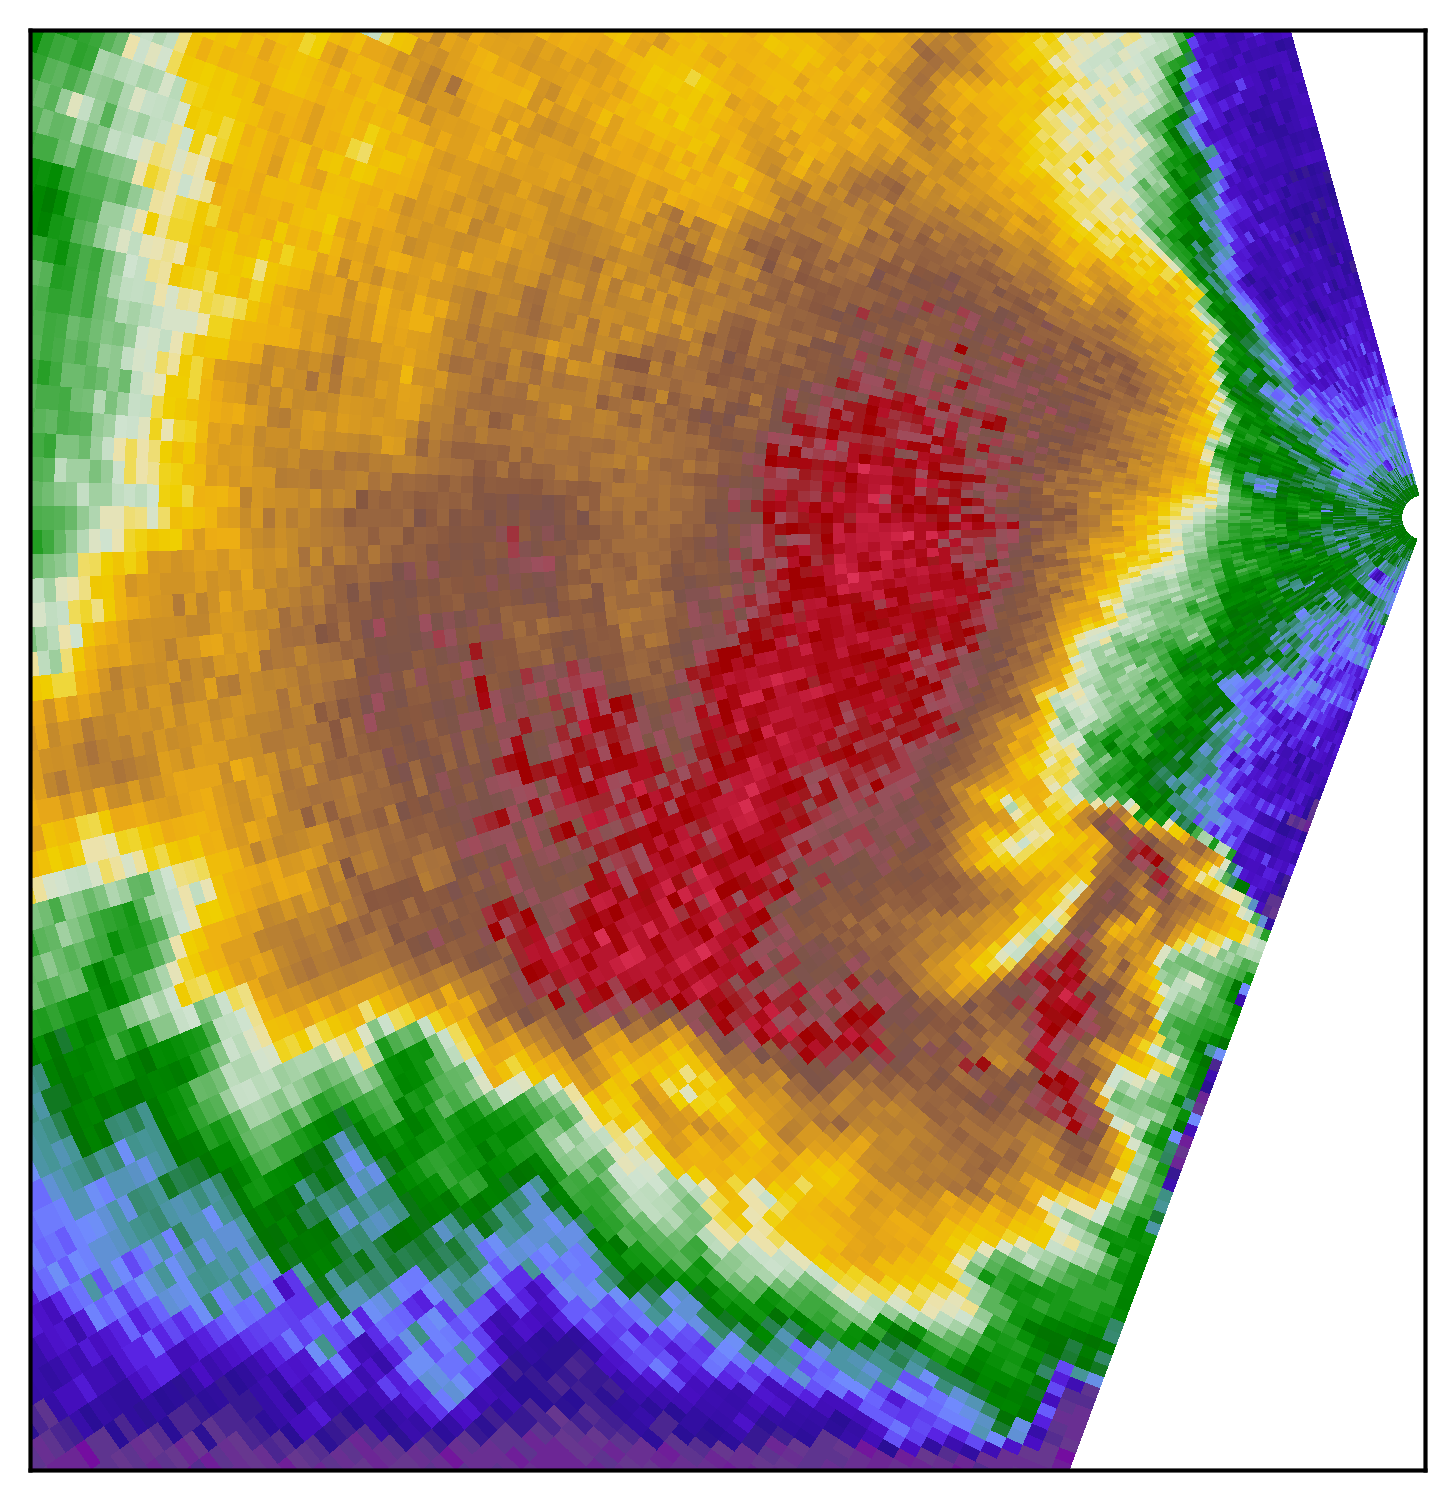
\includegraphics[scale=0.17]{figures/title_ppi.png}}
\logo{
\includegraphics[scale=0.6]{figures/eec_logo_black.png}}

%Python is known for having “batteries included”: a feature-filled standard
%library which reduces development effort for many common tasks, such as logging,
%configuration files, and command line parsing. The utilization of this standard
%library allows the addition of features to software while adding little
%additional code, or even reducing the amount of code for existing software.
%Also, by virtue of its dynamic nature and powerful built-in data structures,
%Python is able to provide a drastically simpler interface for reading NetCDF
%datasets compared to the standard interfaces in languages like C or FORTRAN.
%Python's concept of modules additionally facilitates the creation of small,
%reusable software components, which promotes code reuse. These qualities reduce
%the volume of code that must be developed and maintained, which accelerates the
%development cycle. The porting of a software radar simulator from pure C to a
%mixture of C and Python is used as a case study in the benefits moving software
%to Python.

\begin{document}

\definecolor{keywords}{RGB}{255,0,90}
\definecolor{comments}{RGB}{29,147,48}
\lstset{ %
language=Python,                % choose the language of the code
basicstyle=\ttfamily\scriptsize, % the size of the fonts that are used for the code
%numbers=left,                   % where to put the line-numbers
%numberstyle=\scriptsize,        % the size of the fonts that are used for the line-numbers
%stepnumber=1,                   % the step between two line-numbers. If it's 1 each line
                                % will be numbered
%numbersep=5pt,                  % how far the line-numbers are from the code
backgroundcolor=\color{white},   % choose the background color. You must add \usepackage{color}
showspaces=false,               % show spaces adding particular underscores
showstringspaces=false,         % underline spaces within strings
showtabs=false,                 % show tabs within strings adding particular underscores
frame=single,                   % adds a frame around the code
tabsize=2,                      % sets default tabsize to 2 spaces
captionpos=b,                   % sets the caption-position to bottom
breaklines=true,                % sets automatic line breaking
breakatwhitespace=false,        % sets if automatic breaks should only happen at whitespace
title=\lstname,                 % show the filename of files included with \lstinputlisting;
                                % also try caption instead of title
escapeinside={\%*}{*)},         % if you want to add a comment within your code
morekeywords={*,...}            % if you want to add more keywords to the set
keywordstyle=\color{keywords},
commentstyle=\color{comments}\emph,
linewidth=240pt
}

\frame{\titlepage}

\section[Outline]{}
\begin{frame}{Outline}
    \tableofcontents
\end{frame}

\section{Background}
\stepcounter{subsection}
\begin{frame}[<+->]
  \frametitle{Simulation Software}
  \begin{itemize}
    \item Software simulates radar data from numerical simulation output
    \item Radar data simulated based on configured radar and scanning strategy parameters
    \item Computationally expensive simulation
    \item Desire to utilize as a teaching tool...
    \item ...which implied a need to improve the usability
    \item Before: 5400 LOC C
    \item Now: 2000 LOC Python, 2900 LOC C (+8500 LOC FORTRAN Library)
    \item Time to "python-ize": ~1 month for a single graduate student (me)
  \end{itemize}
\end{frame}

\begin{frame}[<+->]
  \frametitle{Why I Chose Python}
  \begin{itemize}
    \item Had already begun utilizing Python (+ Numpy, Scipy, Matplotlib) in lieu of MATLAB
        for many analysis tasks.
    \item Needed to develop simulation code further and leveraged Python to improve rate of development:
    \begin{itemize}
      \item<3-> Improve command line usability \only<4->{\alert<4>{[optparse]}}
      \item<3-> Vastly improve configuration files \only<5->{\alert<5>{[ConfigParser]}}
      \item<3-> Keep debugging output but hide from users \only<6->{\alert<6>{[logging]}}
      \item<3-> Update the NetCDF code with more output \only<7->{\alert<7>{[pupynere]}}
      \item<3-> Improve scatter calculation code \only<8->{\alert<8>{[existing python code]}}
      \item<3-> Leverage highly optimized computing code \only<9->{\alert<9>{[ctypes]}}
    \end{itemize}
  \end{itemize}
\end{frame}

\section[The Standard Library]{Batteries Included...The Standard Library}
\stepcounter{subsection}
\begin{frame}
  \frametitle{Why is the Standard Library Important?}
  \begin{itemize}
    \item<1-> Libraries you can count on with every installation -> minimal dependency headaches
    \item<2-> Starting point for finding solid libraries to handle given tasks
    \item<3-> Ones used in this code:
      \begin{itemize}
        \item collections, itertools - collecting and looping over items
        \item math - mathematical functions
        \item warnings - issuing and suppressing warnings
        \item os.path - OS-independent path/file-name manipulation
        \item datetime, time, calendar - working with dates and times
        \item \alert<4->{ConfigParser} - configuration file parsing
        \item \alert<4->{optparse} - command-line option parsing
        \item \alert<4->{logging} - controlling output
        \item \alert<4->{ctypes} - calling into libraries
      \end{itemize}
  \end{itemize}
\end{frame}

\begin{frame}
  \frametitle{Configuration Files}
  \begin{itemize}
    \item The radar simulation software makes use of configuration files to
      control various radar operation parameters
    \item Old format read values from a file in fixed order (Text field present for user but not parsed)
    \item Made use of ConfigParser module from the standard library
    \item Provides flexible configuration files with support for sections and comments
    \item Simple API to open a configuration file and begin reading options
  \end{itemize}
\end{frame}

\begin{frame}{<+->}
  \frametitle{Configuration Files:Impacts}
  \begin{itemize}
    \only<1> { \lstinputlisting[caption=]{oldconfig} }
    \only<2> { \lstinputlisting[caption=]{newconfig} }
    \item<3-> Replaced brittle file format with something that is easy for users to understand
    \item<4-> Replaced brittle, unmaintainable code with something much easier to enhance
    \item<5-> Shrank code by 600 LOC
  \end{itemize}
  \uncover<6>{HUGE usability improvment.}
\end{frame}

\begin{frame}
  \frametitle{Logging}
  \begin{itemize}
    \item Console messages are the way the program communicates with the user
    \item However, the messages that are useful to a developer are not the
      same as what other users needs to see
    \item Logging libraries provide custom printing functions that allow fine-grained
      control of what messages are printed
    \item Python includes the {\bf logging} module that includes a raft of features:
    \begin{itemize}
      \item Control of message information (time, filename, line number, etc.)
      \item Different message commands for different levels (warning, info, debug, etc.)
      \item Different message handlers (file, screen, email?)
    \end{itemize}
  \end{itemize}
\end{frame}

\begin{frame}[<+->]
  \frametitle{Logging:Impacts}
  \begin{itemize}
    \item Added 40 LOC to set up logging, replaced prints with logger.*
    \item Can optionally get detailed messages with a simple command line flag
    \item Can turn on some messages only when \emph{I} want them
    \item Can tell messages to log to a file
    \item No \#ifdefs or commenting/uncommenting prints
    \item Big improvements in usability for me as a developer and for other users
  \end{itemize}
\end{frame}

\begin{frame}[fragile]
  \lstset{language=Python}
  \frametitle{Command Line Parser}
  \begin{itemize}
    \item optparse module included in Python standard library
    \item Handle parsing of commandline into passed in arguments and options:

    \verb$radarsim -vvv -d -l run.log config/example.config$
    \item Programmatically add individual options
    \lstinputlisting[caption=]{optparse.py}
    \item Can also set default values for options
    \item Get a help display for free
  \end{itemize}
\end{frame}

\begin{frame}[fragile]{Help Screen}
\tiny
\begin{verbatim}
Usage: radarsim [options] configfiles

Options:
  --version             show program's version number and exit
  -h, --help            show this help message and exit
  -v, --verbose         Produce more verbose messages. Specify more than once
                        for more messages.
  -q, --quiet           Make output messages more quiet. Specify more than
                        once for less output.
  -d, --detailed        Use detailed logging messages.
  -l FILE, --log-output=FILE
                        Log output messages to FILE. Only error messages will
                        be displayed to the console.
  -L, --log-only        Used to specify that output only goes to logfile. Need
                        to also specify --log-output.
\end{verbatim}
\end{frame}

\begin{frame}
  \frametitle{Command Line Parser:Impacts}
  \begin{itemize}
    \item Increased code by 10 LOC
    \item However, old code was simplistic
    \item Those 100 lines of new code added support for:
    \begin{itemize}
      \item Controlling message verbosity
      \item Controlling other logger behavior
      \item Drastically improved help message
    \end{itemize}
  \end{itemize}
  Overall impact was a large increase in usability with minimal development effort.
\end{frame}

\section{NetCDF}
\stepcounter{subsection}
\begin{frame}
  \frametitle{Python NetCDF API}
  \begin{itemize}
    \item<1-> Many packages:
    \begin{itemize}
      \item PyNIO - Part of NCAR's PyNGL package
      \item Scientific.IO.NetCDF
      \item \alert<4> {pupynere (scipy.io.netcdf)}
      \item netcdf4-python
    \end{itemize}
    \item<2-> But they all pretty much follow the same API
    \item<3-> Which is \emph{much} simpler than reading and writing NetCDF in C
  \end{itemize}
\end{frame}

\begin{frame}[fragile]{Comparison: Reading a variable}
  \lstset{language=C}
  \begin{lstlisting}
    int nc_file, var_id, ndims;
    nc_open("Test_data.nc", NC_NOWRITE, &nc_file);
    nc_inq_varid(nc_file, "Temperature", &var_id);
    nc_inq_varndims(nc_file, var_id, &ndims);
    int* dims = malloc(ndims * sizeof(int));
    nc_inq_vardimid(nc_file, var_id, dims);
    size_t dim_len, total_size = 1;
    for(int i=0; i<ndims; ++i)
    {
        nc_inq_dimlen(nc_file, dims[i], &dim_len);
        total_size *= dim_len;
    }
    float* var = malloc(total_size * sizeof(float));
    nc_get_var_float(nc_file, var_id, var);
    free(dims); free(var);
    nc_close(nc_file);
  \end{lstlisting}
\end{frame}

\begin{frame}[fragile]{Comparison: Reading a variable}
  \lstset{language=Python}
  \begin{lstlisting}
  from pupynere import netcdf_file
  nc = netcdf_file('Test_data.nc', 'r')

  temp_var = nc.variables('Temperature')

  print temp_var.units

  nc.close()
  \end{lstlisting}
\end{frame}

\begin{frame}
  \frametitle{Python NetCDF API: Impacts}
  \begin{itemize}
    \item Rewrote I/O layer -- shrank by 800 LOC
    \item Better output metadata (units, time of run, etc.)
    \item Adding new input and output fields/attributes much simpler with Python
    \item As a consequence, the output files contain much more useful
      information for reproducing previous results
  \end{itemize}
\end{frame}

\section[Modularity]{Modularity and Wrapping existing code}
\stepcounter{subsection}
\begin{frame}{Wrapping code}
  \begin{itemize}
    \item<1-> \alert<4->{Ctypes} - wrap existing libraries
    \begin{itemize}
        \item Can express C structures in a python syntax
        \item Dynamically grab function names and specify calling types
        \item Can use pointer types to pass numpy arrays
    \end{itemize}
    \item<2-> \alert<4->{F2Py} - wrap and call FORTRAN code from Python
    \item<3-> Cython - Generate C-code (and compiled library) from Python-like syntax
  \end{itemize}
\end{frame}

\begin{frame}[<+->]{Modular Code Reuse}
  \begin{itemize}
    \item Needed T-Matrix calculations -> F77 Code
    \item Wrapped with F2Py to give a nice NumPy interface for scattering calculations
    \item Used initially just for quick analyses of scattering effects
    \item Was able to re-use this module (which lives as a separate project)
    \item Re-use leads to better testing and fixing as opposed to separate code bases
  \end{itemize}
\end{frame}

\section{Wrapping up}
\stepcounter{subsection}
\begin{frame}[<+->]
  \frametitle{Concluding remarks}
  Python:
  \begin{itemize}
    \item Offers many built-in libraries that can simplify development
    \item Can \emph{drastically} simplify working with NetCDF files
    \item Permits keeping performance-sensitive compiled codes
    \item Promotes through its module system the use and \emph{reuse} of modular code
    \item is \emph{not} necessarily enabling any functionality that could not be done in C or FORTRAN...
    \item ...but makes it much easier
  \end{itemize}
\end{frame}

\begin{frame}
  \frametitle{Thanks and Questions}
  Thanks to:
  \begin{description}[Matplotlib]
    \item[Python]{http://www.python.org}
    \item[NumPy]{http://numpy.scipy.org}
    \item[SciPy]{http://www.scipy.org}
    \item[Matplotlib]{http://matplotlib.sourceforge.net}
    \item[pupynere]{http://pypi.python.org/pypi/pupynere}
  \end{description}
  Questions?
\end{frame}

\end{document}
